% ======================================================================
%  Paper T -- rank-2 selection-rule obstruction to Raman sideband cooling
%  of alkali clock qubits.
%
%  Compile: pdflatex -> bibtex -> pdflatex x2   (or use Overleaf).
%  Figure files needed alongside this .tex (or adjust \graphicspath):
%     fig_rsc_vs_eit.png        (Fig. 2 -- floor comparison; in repo/figures)
%     fig_fom_vs_detuning.png   (Fig. 3 -- FoM vs detuning;   in repo/figures)
%     fig_level_scheme.pdf      (Fig. 1 -- level scheme; in repo/figures)
%
%  STATUS: quantitative sections (III, IV, V, VII), abstract, table, and the
%  FoM box are the verified core (src/paper_T_fom.py, rsc_floor_rate_eqn.py,
%  paper_T_generality.py).  Sections I, II, VI, VIII are first drafts.
%  Author list/order TO BE CONFIRMED with F. Minardi and M. Prevedelli.
% ======================================================================
\documentclass[aps,pra,reprint,amsmath,amssymb,superscriptaddress,floatfix]{revtex4-2}

\usepackage{graphicx}
\usepackage{bm}
\usepackage{braket}
\usepackage{siunitx}
\graphicspath{{./}{figures/}{../../figures/}}

\newcommand{\nbar}{\bar n}
\newcommand{\Dm}{\Delta m}
\newcommand{\dhfs}{\Delta_{\mathrm{HFS}}}
\newcommand{\FoM}{\mathrm{FoM}}

\begin{document}

\title{A rank-2 selection-rule obstruction to Raman sideband cooling of alkali clock qubits}

\author{M.~Dondi}
\email{michelangelo.dondi@unibo.it}
\affiliation{Dipartimento di Fisica e Astronomia, Universit\`a di Bologna, and INFN Sezione di Bologna, I-40127 Bologna, Italy}
% \author{F.~Minardi}\affiliation{...}   % authorship to be confirmed

\date{\today}

\begin{abstract}
Field-insensitive ``clock'' states of alkali atoms---the $m_F$ sublevels with matched
$g_F m_F$---are the natural qubit and metrology basis, but cooling them directly to the motional
ground state is constrained. We show that Raman sideband cooling on a field-insensitive clock pair
of $^{87}$Rb is obstructed by a selection rule: connecting the pair with a single two-photon
momentum kick requires a $\Dm=2$ (rank-2) operator, and the rank-2 component of a two-photon
operator vanishes identically in a $J=\tfrac12$ ground manifold, since the reduced matrix element
requires the forbidden triangle $(\tfrac12,2,\tfrac12)$. The transition survives only through
excited-state hyperfine mixing, with amplitude $\propto\dhfs/\Delta^2$, so the coherence per
spontaneously scattered photon is pinned at a figure of merit of order $\dhfs/\Gamma\approx5$---
independent of detuning, and unimprovable. A Lamb--Dicke rate analysis gives a cooling floor
$\nbar\approx0.45$, robust to a factor-three change in the scattering prefactor.
Electromagnetically-induced-transparency cooling on the same pair evades the obstruction by
operating near resonance, reaching $\nbar\approx0.005$. Extending the analysis across the alkali
series, the obstruction is universal and is in fact strongest for the light alkalis, where the
figure of merit falls below unity. The result identifies a general constraint on direct sideband
cooling of alkali clock qubits and singles out EIT as the field-insensitive route.
\end{abstract}

\maketitle

% ======================================================================
\section{Introduction}
% ----------------------------------------------------------------------
Preparing trapped neutral atoms in the motional ground state underlies optical-clock accuracy,
high-fidelity qubit operations, and the coherent transport of atoms in tweezers, lattices, and
hollow-core fibres. The states one most wants to cool are the \emph{clock} states: the
hyperfine-Zeeman sublevels whose energy difference is first-order insensitive to magnetic field,
realized either by the $m_F=0$ pair or, more generally, by a pair of sublevels with matched
$g_F m_F$. These are the states in which coherence is stored and metrology is performed, so cooling
them \emph{directly}---rather than cooling an auxiliary cycling state and inheriting its
motion---is attractive.

Raman sideband cooling (RSC) is the standard tool. A pair of laser fields drives a stimulated
two-photon transition that removes one motional quantum, and an incoherent repump recycles the
internal state; iterated, the atom is pumped toward the dark motional ground state. RSC is fast,
deep, and routinely reaches $\nbar\ll1$ on suitable transitions. It is therefore natural to ask
whether one can simply apply RSC to a field-insensitive clock pair.

Here we show that, for alkali atoms, one cannot. The geometry that imparts a single motional
quantum along the trap axis with a guided or retroreflected beam pair forces the clock-pair Raman
to be a $\Dm=2$ transition, and a $\Dm=2$ two-photon operator is a rank-2 spherical tensor whose
matrix element vanishes identically within a $J=\tfrac12$ ground manifold. The transition is not
forbidden outright---it is recovered through excited-state hyperfine mixing---but only with an
amplitude suppressed by the ratio of the excited-state hyperfine splitting to the detuning. The
consequence is a hard ceiling on the coherence accumulated per spontaneously scattered photon
that, crucially, \emph{cannot be improved by detuning}, and that leaves the cooling floor far
above the ground state. We compute the obstruction from first principles
(Sec.~\ref{sec:obstruction}), derive the figure-of-merit ceiling and its detuning-independence
(Sec.~\ref{sec:fom}), translate it into a cooling floor (Sec.~\ref{sec:floor}), contrast it with
electromagnetically-induced-transparency (EIT) cooling on the \emph{same} pair
(Sec.~\ref{sec:eit}), and show that the obstruction is universal across the alkali series
(Sec.~\ref{sec:generality}).

% ======================================================================
\section{The clock pair and the $\Dm=2$ requirement}\label{sec:clockpair}
% ----------------------------------------------------------------------
We take $^{87}$Rb as the concrete example; the generalization is given in
Sec.~\ref{sec:generality}. The ground manifold is $5S_{1/2}$ ($J=\tfrac12$, $I=\tfrac32$), with
hyperfine levels $F=1,2$. Consider the pair
\begin{equation}
g_1=\ket{F{=}1,m_F{=}{-}1},\qquad g_2=\ket{F{=}2,m_F{=}{+}1}.
\end{equation}
Both have $g_F m_F=+\tfrac12$ (using $g_{F=2}=+\tfrac12$, $g_{F=1}=-\tfrac12$), so their energy
difference is first-order insensitive to magnetic field at \emph{any} field strength, and the pair
is immune to the first-order vector light shift. It is thus a genuine field-insensitive clock
qubit, unlike the stretched pair $\ket{2,+2}/\ket{2,+1}$, which is field-sensitive and not a clock
pair.

To cool the axial motion with a single guided beam and its retroreflection (or two beams sharing
the trap axis), the two Raman photons are delivered with opposite helicity along the quantization
axis---one $\sigma^+$, one $\sigma^-$---so that the net change in magnetic quantum number is
$\Dm=m_{F,2}-m_{F,1}=+2$. Connecting a field-insensitive alkali clock pair with a single
axial two-photon kick is, generically, a $\Dm=2$ operation. This is the geometric fact whose
consequences we now examine.

% ======================================================================
\section{The rank-2 obstruction}\label{sec:obstruction}
% ----------------------------------------------------------------------
Adiabatically eliminating the excited manifold, the effective two-photon coupling between the
ground states is
\begin{equation}
T_{\mathrm{eff}}=\sum_e\frac{(\bm d\!\cdot\!\bm\varepsilon_2)\,\ket{e}\bra{e}\,(\bm d\!\cdot\!\bm\varepsilon_1)}{\Delta_e},
\end{equation}
with $\bm\varepsilon_{1,2}$ the beam polarizations and $\Delta_e$ the one-photon detuning from
$\ket{e}$. The product of two rank-1 dipole operators decomposes into irreducible tensors of rank
$K=0,1,2$; for $\Dm=2$ only $K=2$ contributes. Writing the two-photon Rabi frequency as
\begin{equation}\label{eq:omega2ph}
\Omega_{2\mathrm{ph}}(\Delta)=\frac{\bar\Omega_1\bar\Omega_2}{2}\,G(\Delta),\qquad
G(\Delta)=\sum_{F'}\frac{g_{F'}}{\Delta+\delta_{F'}},
\end{equation}
where $\bar\Omega_i$ are the reduced single-photon Rabi frequencies, $\delta_{F'}$ the
excited-state hyperfine shifts, and
\begin{equation}
g_{F'}=\bra{2,1}d_{+1}\ket{F',0}\bra{F',0}d_{+1}\ket{1,-1},
\end{equation}
the reduced line strength $\braket{J'\Vert d\Vert J}$ factors out and cancels in every ratio below.
Only $F'=1,2$ contribute; the remaining $F'$ have a vanishing leg by the dipole triangle rule.

The rank-2 component of a two-photon operator cannot act within a spin-$\tfrac12$ manifold: a
$J=\tfrac12$ space supports no rank-2 spherical tensor, equivalently
$\braket{J{=}\tfrac12\Vert T^{(2)}\Vert J{=}\tfrac12}$ requires the triangle $(\tfrac12,2,\tfrac12)$,
i.e. $0\le2\le1$, which fails. In the degenerate-excited limit $\delta_{F'}\!\to\!0$, the amplitude
collapses to this matrix element and therefore vanishes identically,
\begin{equation}\label{eq:null}
\boxed{\;\sum_{F'} g_{F'} = 0\;}
\end{equation}
With the dipole acting only on the electronic coordinate, the angular factors evaluate in closed
form to
\begin{equation}
g_{1}=-g_{2}=-\frac{1}{4\sqrt3}\approx-0.1443
\end{equation}
in units of $\braket{J'\Vert d\Vert J}^2$, so Eq.~\eqref{eq:null} holds exactly. The level scheme
and the cancelling pair of paths are shown in Fig.~\ref{fig:levels}.

\begin{figure}[t]
\centering
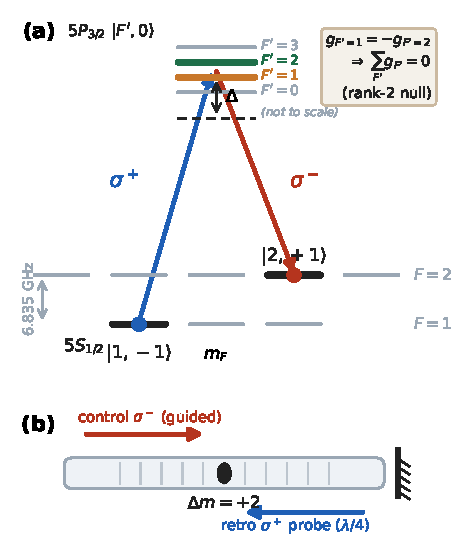
\includegraphics[width=\columnwidth]{fig_level_scheme.pdf}
\caption{\label{fig:levels} (a)~Level scheme of the $\Dm=2$ field-insensitive clock-pair Raman in
$^{87}$Rb: $\ket{1,-1}\xrightarrow{\sigma^+}\ket{F',0}$ of $5P_{3/2}\xrightarrow{\sigma^-}\ket{2,+1}$,
both legs through $m'=0$. The two contributing excited levels $F'=1,2$ carry opposite-sign
amplitudes ($g_1=-g_2$), i.e. the rank-2 null $\sum_{F'}g_{F'}=0$. (b)~Mirror-ladder geometry: a
guided $\sigma^-$ control and a retroreflected $\sigma^+$ probe along the trap axis deliver a single
$\Dm=+2$ two-photon kick.}
\end{figure}

% ======================================================================
\section{The coherence-per-scatter ceiling}\label{sec:fom}
% ----------------------------------------------------------------------
The excited-state hyperfine splittings break the cancellation in Eq.~\eqref{eq:null}. Expanding
Eq.~\eqref{eq:omega2ph} for $\Delta\gg\delta_{F'}$ and using $\sum_{F'}g_{F'}=0$,
\begin{equation}\label{eq:survivor}
G(\Delta)\;\to\;-\frac{1}{\Delta^2}\sum_{F'}g_{F'}\delta_{F'}\equiv-\frac{G_2}{\Delta^2},\qquad
G_2=g_1(\delta_1-\delta_2),
\end{equation}
so the surviving amplitude is proportional to the $F'{=}1$--$F'{=}2$ splitting of $5P_{3/2}$
($\delta_1-\delta_2=156.9$~MHz); numerically $G_2=22.7$~MHz and
$\Omega_{2\mathrm{ph}}\propto\dhfs/\Delta^2$.

The off-resonant scattering rate, by contrast, carries the ordinary $1/\Delta^2$ with no rank-2
suppression (scattering is incoherent):
\begin{equation}
R_{\mathrm{sc}}(\Delta)=\Gamma\Big(\tfrac{\bar\Omega}{2}\Big)^2\frac{\Sigma}{\Delta^2},\qquad
\Sigma=\sum_{F'}\big(|c^{(1)}_{F'}|^2+|c^{(2)}_{F'}|^2\big),
\end{equation}
with $c^{(1)}_{F'}=\bra{F',0}d_{+1}\ket{1,-1}$ and $c^{(2)}_{F'}=\bra{F',0}d_{-1}\ket{2,1}$ the
excitation amplitudes of the two clock states. The coherence accumulated per spontaneously
scattered photon is then
\begin{equation}\label{eq:fom}
\boxed{\;\FoM\equiv\frac{\Omega_{2\mathrm{ph}}}{R_{\mathrm{sc}}}
=\frac{2\,|G_2|}{\Gamma\,\Sigma}\;\propto\;\frac{\dhfs}{\Gamma}\;}
\end{equation}
The $\Delta^2$ cancels: the figure of merit is \emph{independent of detuning}. Numerically
$\FoM\approx5.6$ radians of two-photon rotation per scattered photon ($\Sigma=4/3$,
$\Gamma/2\pi=6.07$~MHz)---one cannot complete even a single sideband $\pi$-pulse without scattering
$\sim0.5$ photon.

An \emph{allowed} Raman ($\Dm\le1$, no null) has $\Omega_{2\mathrm{ph}}\propto1/\Delta$ and thus
$\FoM\propto\Delta/\Gamma$, improvable without bound by detuning---the standard far-detuned Raman
strategy. The $\Dm=2$ clock Raman cannot be detuned out of trouble: signal and scatter fall at the
same rate, and the ceiling is fixed at $\sim\dhfs/\Gamma\sim$~a few. The two scalings are compared
in Fig.~\ref{fig:fomvsdetuning}.

\begin{figure}[t]
\centering
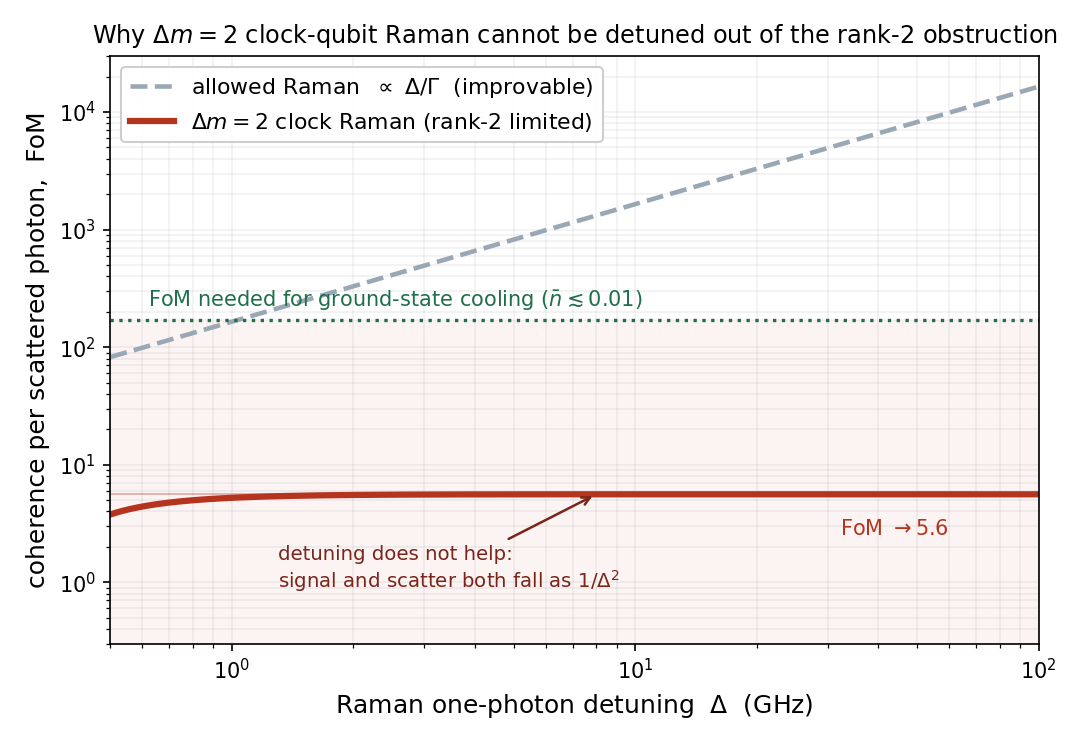
\includegraphics[width=\columnwidth]{fig_fom_vs_detuning.png}
\caption{\label{fig:fomvsdetuning} Coherence per scattered photon versus Raman detuning. The
$\Dm=2$ clock Raman (rank-2 limited) is flat at $\FoM\approx5.6$ across four decades of detuning,
while an allowed Raman improves as $\Delta/\Gamma$. Neither reaches the $\FoM\gtrsim170$ required
for ground-state cooling (Sec.~\ref{sec:floor}); the allowed curve crosses it near $\Delta=1$~GHz,
the $\Dm=2$ curve never does.}
\end{figure}

% ======================================================================
\section{The cooling floor}\label{sec:floor}
% ----------------------------------------------------------------------
The bounded figure of merit feeds a standard Lamb--Dicke rate equation. Driving the red sideband
with repump dissipation, the steady state is $\nbar_{\rm ss}=A_+/(A_--A_+)$, with cooling rate
$A_-=\eta_{\rm sb}^2\,\Omega_2/\Gamma_{\rm eff}$ (the repump-broadened red sideband) and heating
$A_+=R_{\rm sc}\,\eta_{\rm rec}^2$ from the off-resonant Raman-beam scatter, where
$\eta_{\rm rec}^2=\eta_{780}^2+\eta_{\rm em}^2$ is the recoil per scattered photon. Writing
$r=\Gamma_{\rm eff}/\Omega_2$ (the repump-to-Raman ratio) and $R_{\rm sc}=\Omega_2/\FoM$,
\begin{equation}\label{eq:nbar}
\nbar_{\rm ss}=\frac{\eta_{\rm rec}^2/\FoM}{\;\eta_{\rm sb}^2/r-\eta_{\rm rec}^2/\FoM\;}.
\end{equation}
At the obstruction-bounded $\FoM\approx5.6$ this is of order $0.1$--$1$; for example
$\nbar=0.43$ at $r=5$ ($T_z\approx19\,\mu$K, $70\%$ ground-state population). The absolute value
carries a factor of uncertainty through $r$, but two features are robust: (i) $\nbar=O(0.1$--$1)$,
far above the obstruction-free idealization $\nbar\to10^{-3}$ recovered as $\FoM\to\infty$ (the
regime a standard sideband-cooling model returns when the rank-2 suppression and the
Raman-beam scatter are omitted), and (ii) reaching a useful floor $\nbar\approx0.01$ would require
$\FoM\gtrsim170$---a factor $\sim30$ beyond the $J=\tfrac12$, $\Dm=2$ ceiling. The $\Dm=2$ clock
Raman is therefore disqualified for ground-state cooling. Figure~\ref{fig:floor} places the floor
beside the EIT and stretched-state results.

\begin{figure}[t]
\centering
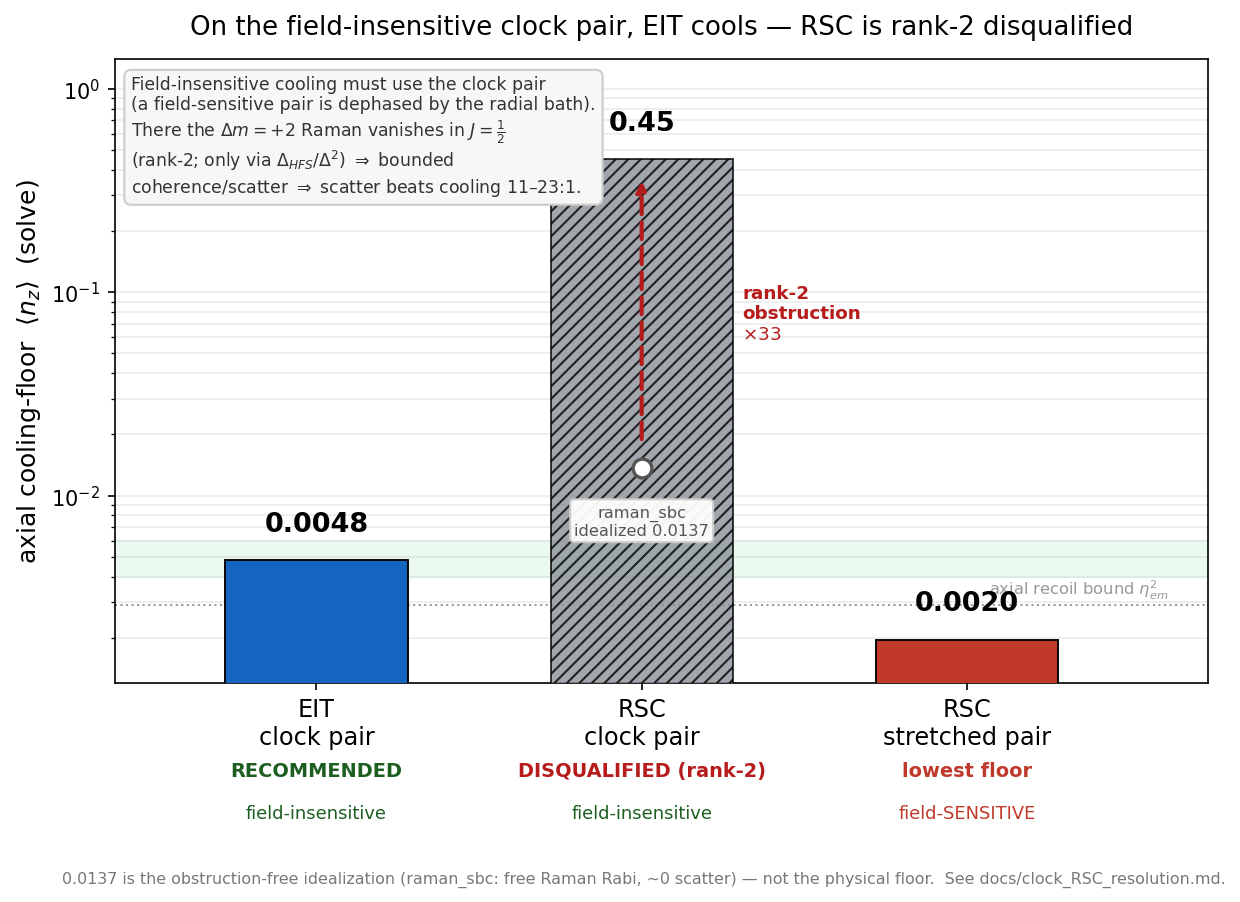
\includegraphics[width=\columnwidth]{fig_rsc_vs_eit.png}
\caption{\label{fig:floor} Steady-state $\nbar$ for cooling the $^{87}$Rb axial mode: EIT on the
field-insensitive clock pair ($\nbar\approx0.005$); $\Dm=2$ Raman sideband cooling on the same
pair (disqualified, $\nbar\approx0.45$, rank-2 limited), with the obstruction-free idealization
marked; and Raman cooling on the field-sensitive stretched pair for reference.}
\end{figure}

% ======================================================================
\section{Contrast: EIT cooling evades the obstruction}\label{sec:eit}
% ----------------------------------------------------------------------
The obstruction is specific to the \emph{far-detuned} operation of RSC. EIT cooling
\cite{morigi2000} operates near resonance, where the excited-state hyperfine structure is resolved
and the dark-state cooling does not rely on a far-detuned $\Dm=2$ Raman amplitude; the spontaneous
scattering that limits it is built into the steady state rather than appearing as an
uncompensated loss. On the \emph{same} field-insensitive clock pair, a steady-state solution of the
EIT cooling dynamics yields $\nbar\approx0.0048$ (symmetric two-beam delivery) to $0.0072$
(single-end tagged delivery)---roughly two orders of magnitude below the RSC floor
(Fig.~\ref{fig:floor}). One cannot simply pull the Raman beams near resonance to raise the figure
of merit: the off-resonant scattering then diverges and the very ratio of Eq.~\eqref{eq:fom} is
lost. EIT is the structured near-resonant solution, using dark-state interference rather than large
detuning to suppress heating, and it is the field-insensitive route to the motional ground state.

% ======================================================================
\section{Generality across the alkalis}\label{sec:generality}
% ----------------------------------------------------------------------
The null Eq.~\eqref{eq:null} is a property of the $J=\tfrac12$ ground manifold and therefore holds
for every alkali. The field-insensitive clock pair is universally
$\ket{F{=}I-\tfrac12,-1}/\ket{F{=}I+\tfrac12,+1}$ (matched $g_F m_F$ at any field); only the two
excited levels $F'=I\mp\tfrac12$ carry the surviving amplitude; and $\sum_{F'}g_{F'}=0$ identically
(verified for $I=\tfrac32$ through $\tfrac72$). The asymptotic scatter line strength is an angular
constant $\Sigma_\infty=\tfrac43$ independent of $I$, and the coherent factor $|g_{\rm lo}|$ varies
only weakly ($1/(4\sqrt3)=0.144$ at $I=\tfrac32$; $0.161$ at $I=\tfrac72$). Hence
\begin{equation}
\FoM=\frac{2|g_{\rm lo}|\,\Delta_{F'}}{\Gamma\,\Sigma_\infty},
\end{equation}
fixed per species only by the excited-state $F'{=}(I{-}\tfrac12)\!\leftrightarrow\!(I{+}\tfrac12)$
hyperfine interval $\Delta_{F'}$ and the $D_2$ linewidth $\Gamma$
(Table~\ref{tab:generality}).

\begin{table}[t]
\caption{\label{tab:generality} The $\Dm=2$ clock-Raman figure of merit across the alkalis. The
null $\sum_{F'}g_{F'}=0$ is exact for all; the excited-state $nP_{3/2}$ hyperfine intervals
$\Delta_{F'}$ and linewidths $\Gamma$ are standard tabulated values
\cite{steck_rb,steck_cs,steck_na,tiecke_k,gehm_li}. ``Scatter per $\pi$'' is $\pi/\FoM$.}
\begin{ruledtabular}
\begin{tabular}{lcccc}
atom & $nP_{3/2}$ & $\Delta_{F'}$ (MHz) & $\Gamma/2\pi$ (MHz) & $\FoM$ \\
\colrule
$^{87}$Rb  & $5P_{3/2}$ & 156.9 & 6.07 & 5.6 \\
$^{133}$Cs & $6P_{3/2}$ & 201.3 & 5.22 & 9.3 \\
$^{23}$Na  & $3P_{3/2}$ & 34.3  & 9.79 & 0.76 \\
$^{39}$K   & $4P_{3/2}$ & 9.4   & 6.04 & 0.34 \\
$^{7}$Li   & $2P_{3/2}$ & 5.9   & 5.87 & 0.22 \\
\end{tabular}
\end{ruledtabular}
\end{table}

The ceiling spans $\FoM\approx0.2$ (Li) to $\approx9$ (Cs)---none within a factor $\sim20$ of the
$\gtrsim170$ needed for ground-state cooling, and for the light alkalis (Na, K, Li) it is
\emph{below unity}: more than one photon is scattered per radian of two-photon rotation. Because
$\Delta_{F'}$ shrinks down the series while $\Gamma$ does not, the obstruction bites hardest for
the lightest alkalis. EIT cooling is the field-insensitive route for all of them.

We emphasize that the obstruction is specific to the $J=\tfrac12$ ground manifold of the alkalis.
Alkaline-earth and alkaline-earth-like clock species (Sr, Yb, Ca$^+$, \ldots) have a $J=0$ ground
state with no rank-2 issue, and sideband cooling there proceeds on a resolved narrow line; that
regime is unaffected by the present result.

% ======================================================================
\section{Conclusion}\label{sec:conclusion}
% ----------------------------------------------------------------------
A selection rule, not an engineering limitation, blocks direct $\Dm=2$ Raman sideband cooling of
alkali clock qubits. The $\Dm=2$ two-photon operator required by the single-axis geometry is a
rank-2 tensor that vanishes in the $J=\tfrac12$ ground manifold; the transition is recovered only
through excited-state hyperfine mixing, with an amplitude $\propto\dhfs/\Delta^2$ that pins the
coherence per scattered photon at $\sim\dhfs/\Gamma$, independent of detuning and of order a few.
The resulting cooling floor sits far above the motional ground state for every alkali, and below
unity figure of merit for the light alkalis. Electromagnetically-induced-transparency cooling,
operating near resonance, evades the obstruction and is the field-insensitive route to the ground
state. The same argument bounds any scheme that attempts to drive a $\Dm=2$ transition coherently
within a $J=\tfrac12$ manifold by far-detuned two-photon means.

\begin{acknowledgments}
% TODO: funding, group, discussions.
\end{acknowledgments}

\appendix
% ======================================================================
\section{Product-basis evaluation of the angular factors}\label{app:angular}
% ----------------------------------------------------------------------
The angular factors $g_{F'}$ are evaluated most transparently in the
$\ket{m_J,m_I}$ product basis, where the dipole acts only on the electronic projection
($\Delta m_I=0$ at each vertex):
\begin{widetext}
\begin{equation}
\bra{F_e,m_e}d_q\ket{F_g,m_g}=\sum_{m_J,m_I}
\Braket{J' (m_J{+}q),I m_I | F_e m_e}\,
\Braket{J m_J,I m_I | F_g m_g}\,
\Braket{J m_J;1 q | J'(m_J{+}q)},
\end{equation}
\end{widetext}
times the common $\braket{J'\Vert d\Vert J}$. Each $g_{F'}$ is thus a sum of products of three
Clebsch--Gordan coefficients, and the null $\sum_{F'}g_{F'}=0$ is a Clebsch--Gordan sum rule
expressing the absence of a rank-2 tensor on $J=\tfrac12$. The closed forms quoted in the text and
the values in Table~\ref{tab:generality} are obtained this way.

\bibliography{paper_T}

\end{document}
